\section{Results and discussion of different methods} \label{sec:condes:discussion}

After designing the controllers, their characteristics should be discussed.
This is the aim of this chapter.
\autoref{tab:condes:results:complete} summarizes all conducted experiments to test the controller.
A complete visual summary of all results is provided in the appendix (\autoref{app:cl_results}).


\begin{table}[H]
    \caption{All conducted experiments with the most important values for controller design and disturbances.}
    \centering
    \begin{tabular}{ccccccccc} \toprule
        No. & \multicolumn{3}{c}{Wind} & \multicolumn{2}{c}{$PID_{11}$} & \multicolumn{2}{c}{$PID_{22}$} & System \\ 
          &  $t_{step}$ [\si{\second}] & $ \Delta v_{wind}$ [\si{\metre\per\second}] & $\xi$ [\si{\metre\per\second}]    & Method  &  $v_{wind}$ [\si{\metre\per\second}] & Method  &  $v_{wind}$ [\si{\metre\per\second}]  \\ \midrule
        1 & 0 & 0 & 0 & ZN-maxS & 8 & T-sum & 8 & 8\\ 
        2 & 0 & 0 & 0 & ZN-2p   & 8 & T-sum & 8 & 8\\ 
        3 & 0 & 0 & 0 & ZN-maxS & 8 & T-sum & 8 & 7\\ 
        4 & 0 & 0 & 0 & ZN-2p   & 8 & T-sum & 8 & 7\\
        5 & 0 & 0 & 0.05 & ZN-maxS & 8 & T-sum & 8 & 8\\ 
        6 & 0 & 0 & 0.05 & ZN-2p   & 8 & T-sum & 8 & 8\\
        7 & 1200 & 1 & 0.05 & ZN-maxS & 8 & T-sum & 8 & 8\\ 
        8 & 1200 & 1 & 0.05 & ZN-2p   & 8 & T-sum & 8 & 8\\
        9 & 1200 & 0.1 & 0.005 & ZN-maxS & 8 & T-sum & 8 & 8\\ 
        10 & 1200 & 0.1 & 0.005 & ZN-2p   & 8 & T-sum & 8 & 8\\ \bottomrule
    \end{tabular}
    \label{tab:condes:results:complete}
\end{table}

Experiment Number 8 can be described as follows:
For the input-output pair 1-1 ($PID_{11}$) a controller designed with two-point approximation and Ziegler-Nichols and a PID controller for output pair 2-2 designed by the T-sum method are tested.
Both controller are designed for a wind speed of \SI{8}{\metre\per\second} and tested on the system identified at a wind speed of \SI{8}{\metre\per\second}.
The wind is used as a disturbance and has a maximum noise power $\xi$ of \SI{0.05}{\metre\per\second} and a step of magnitude \SI{1}{\metre\per\second} at $t=\SI{1000}{\second}$. 


\subsection{Comparing with a benchmark}

Fragoso et~al. (\cite[p. 14, Figure 13]{Fragoso_et_al_2017}) is used as a \textit{benchmark}.
To reproduce this figure two set-point changes are applied.
First, at $t=\SI{100}{\second}$ a set-point change of magnitude $A_{P_g}=\SI{-1}{\watt}$ is applied to the generated power $P_g$.
Second, at $t=\SI{800}{\second}$ a set-point change of magnitude $A_{\omega_r}=\SI{-200}{rmp}$ is applied to the rotational speed of the blade $\omega_r$.
The effects on pitch angle $\beta$ and duty cycle $\alpha$ are observed.

\autoref{fig:condes:results:benchmark_compare} shows that Ziegler-Nichols methods design a controller capable of controlling the system.
For the max-slope method a oscillating behaviour around the set-point can be seen (\autoref{fig:condes:results:exp1:ref}) for the rotational speed $\omega_r$ after the set-point change.
The set-point change in generated power $P_g$ shows less disturbance but also some oscillation around the new set-point.

\begin{figure}[H]
    \center
    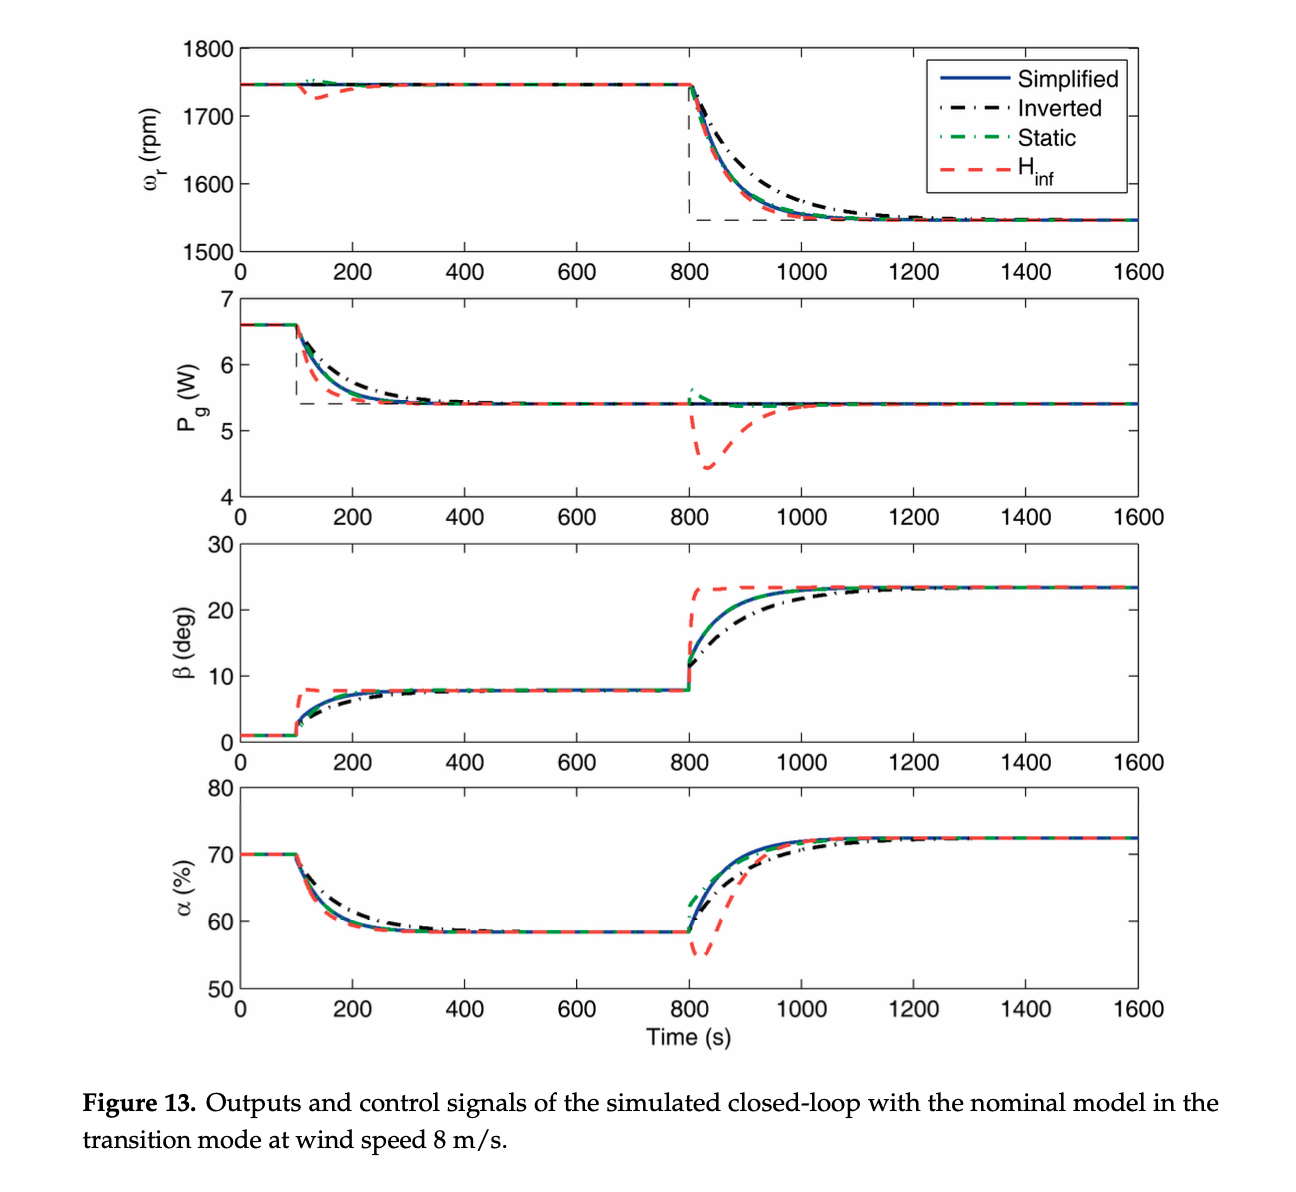
\includegraphics[width=1\textwidth,scale=1,trim=0 0 0 0,clip]{fig/Fragoso_et_al_2017_fig13.png}
    \caption{Figure by \cite{Fragoso_et_al_2017} used as a benchmark process for designed controllers.}
    \label{fig:condes:results:benchmark}
\end{figure}


For the duty cycle $\alpha$ the controller output is not saturated. 
In contrast the pitch angle $\beta$ is heavily saturated.
This shows that the controller is mainly trying to steer the system via the pitch angle, when the rotational speed is changed.
The behaviour is consistent with the predicted behaviour by the relative gain array.  

\begin{figure}[H]
    \centering

    \subcaptionbox{Exp. 1: Wind disturbance, rotational speed of blade and power consumption over time \label{fig:condes:results:exp1:ref}}[.45\textwidth]{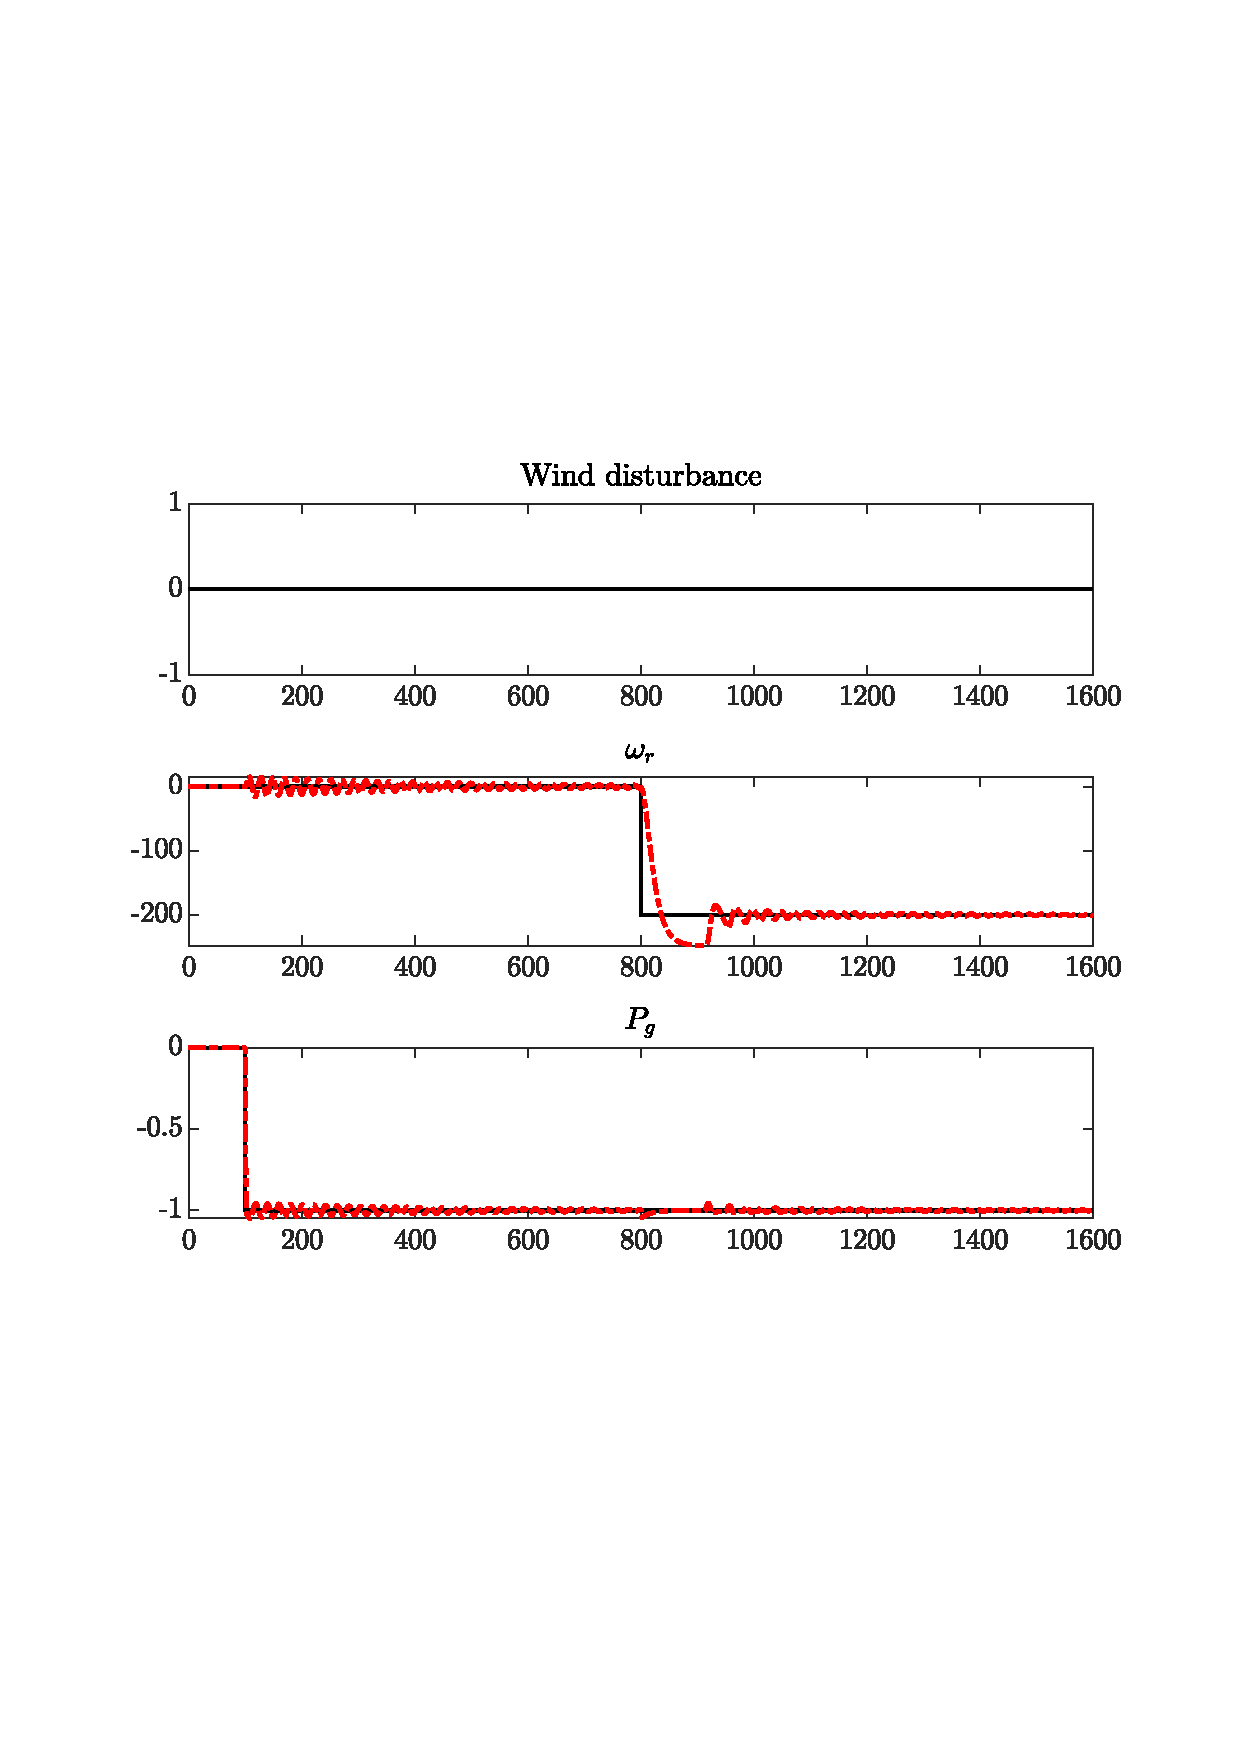
\includegraphics[width=1\linewidth, scale=1, trim=60 230 55 150,clip]{fig/Open_loop/exp_1_ref.pdf}}
%
\subcaptionbox{Exp. 2: Wind disturbance, rotational speed of blade and power consumption over time.\label{fig:condes:results:exp2:ref}}[.45\textwidth]{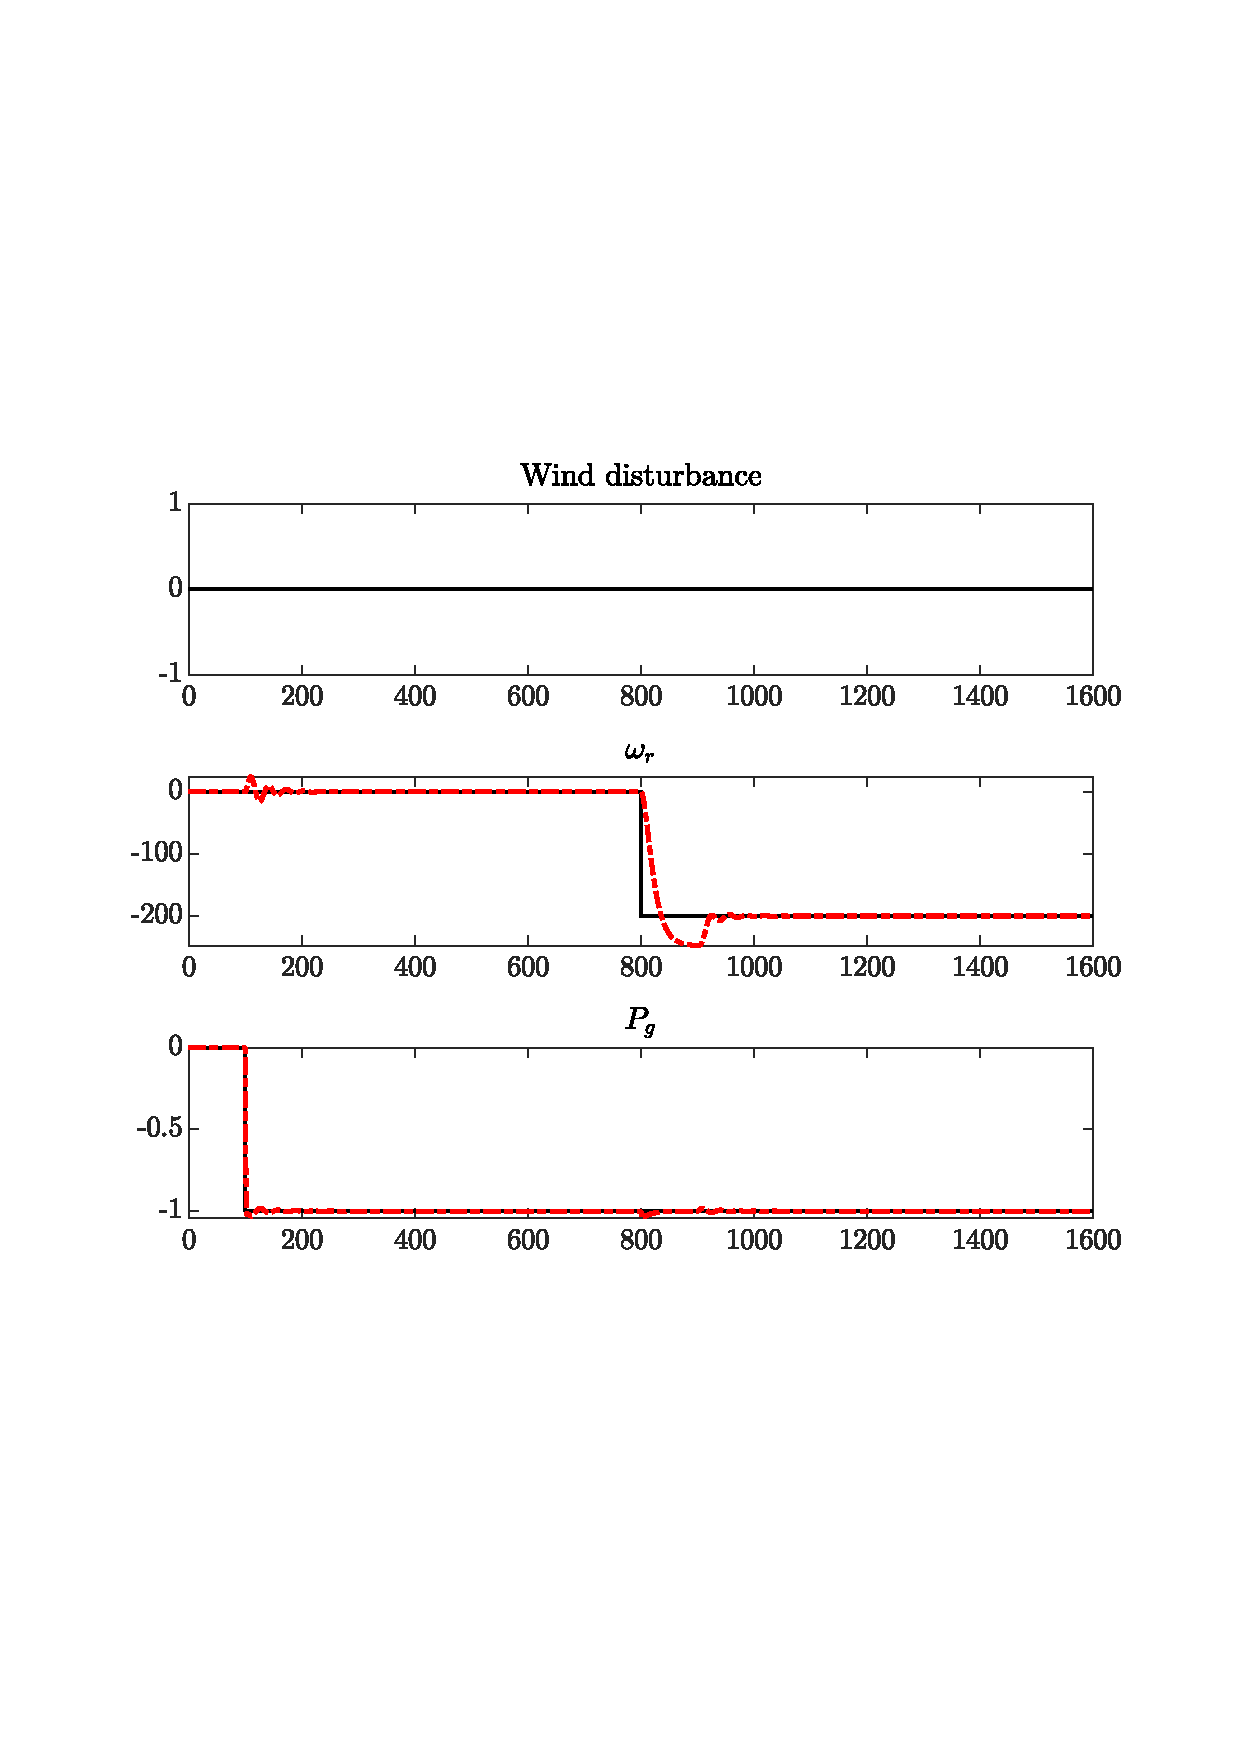
\includegraphics[width=1\linewidth, scale=1, trim=60 230 55 150,clip]{fig/Open_loop/exp_2_ref.pdf}}
\\
    \subcaptionbox{Exp. 1: Blade pitch angle and duty cycle over time before and after saturation. \label{fig:condes:results:exp1:in}}[.45\textwidth]{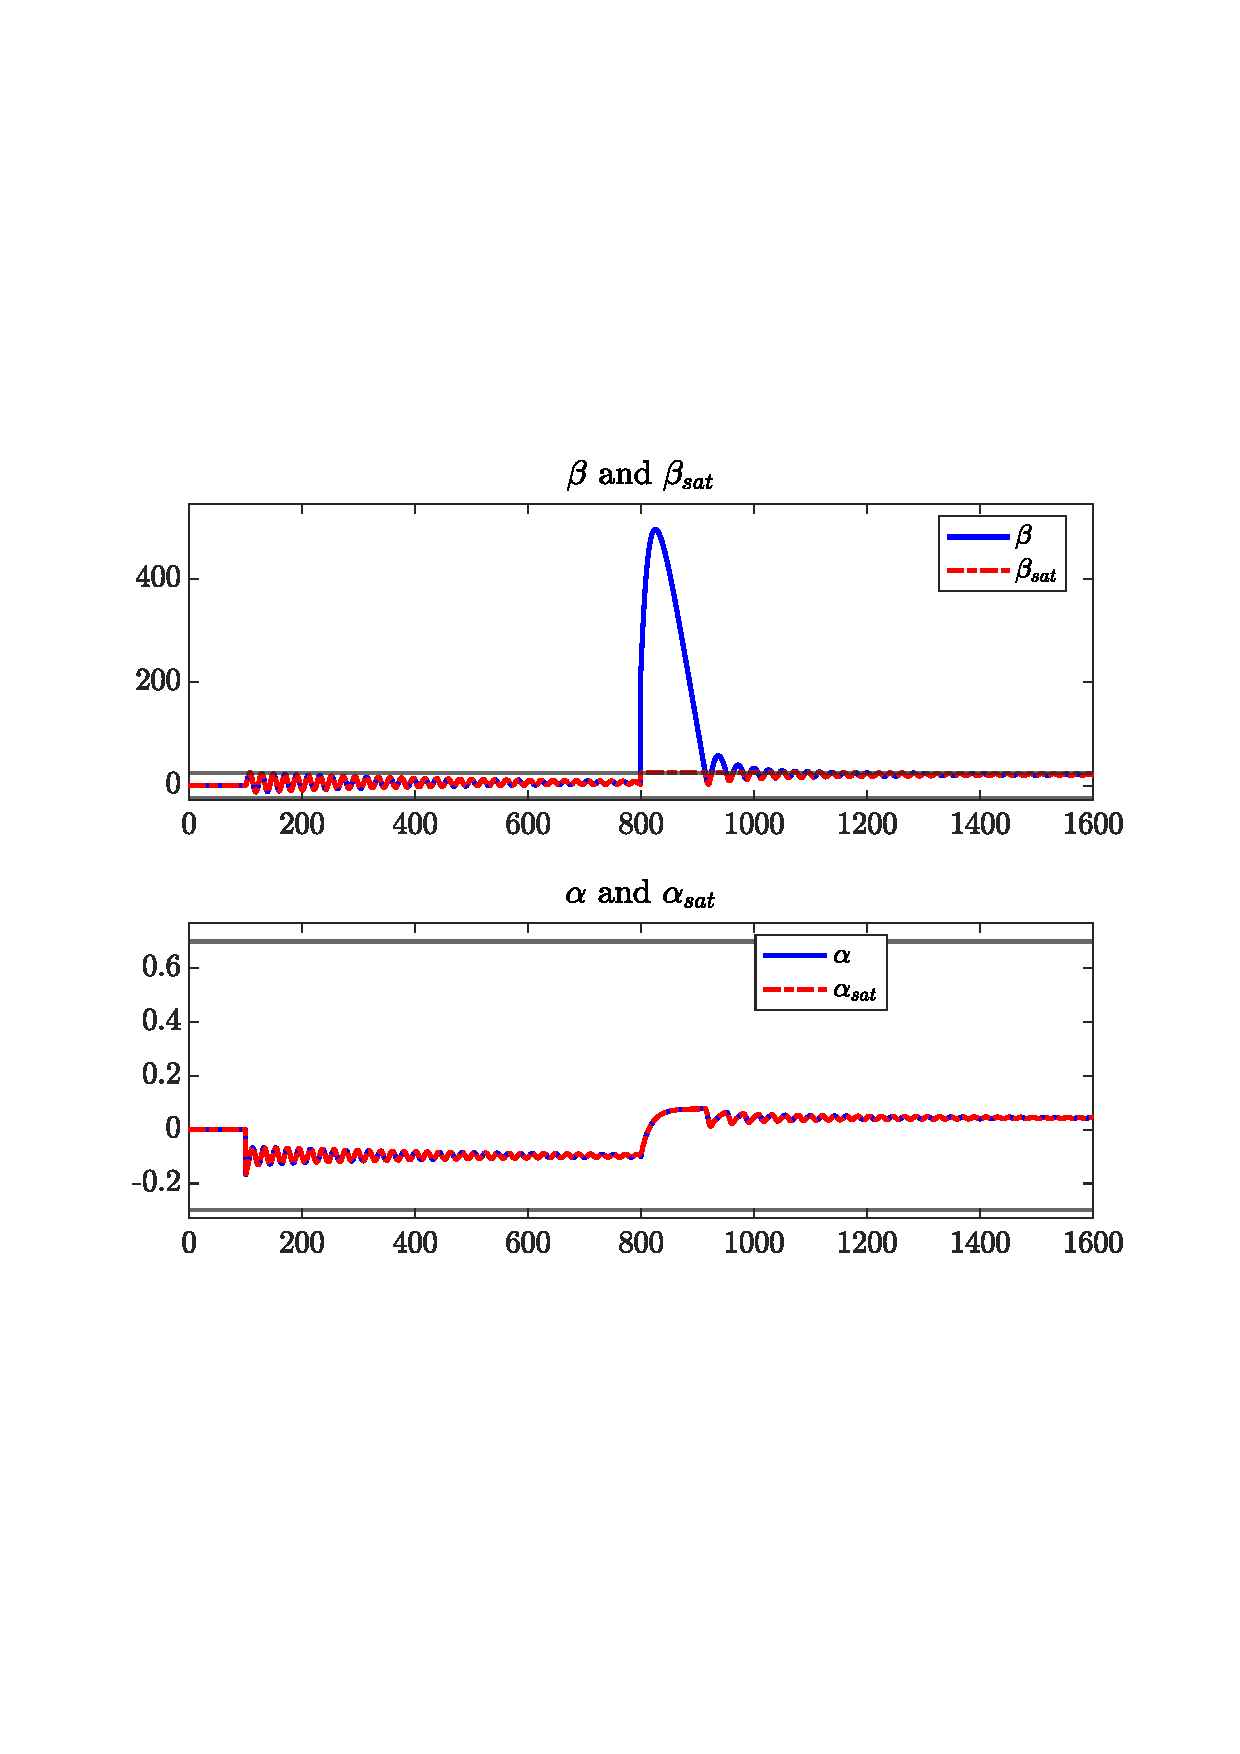
\includegraphics[width=1\linewidth, scale=1, trim=60 230 55 150,clip]{fig/Open_loop/exp_1_in.pdf}}
%
\subcaptionbox{Exp. 2: Blade pitch angle and duty cycle over time before and after saturation. \label{fig:condes:results:exp2:in}}[.45\textwidth]{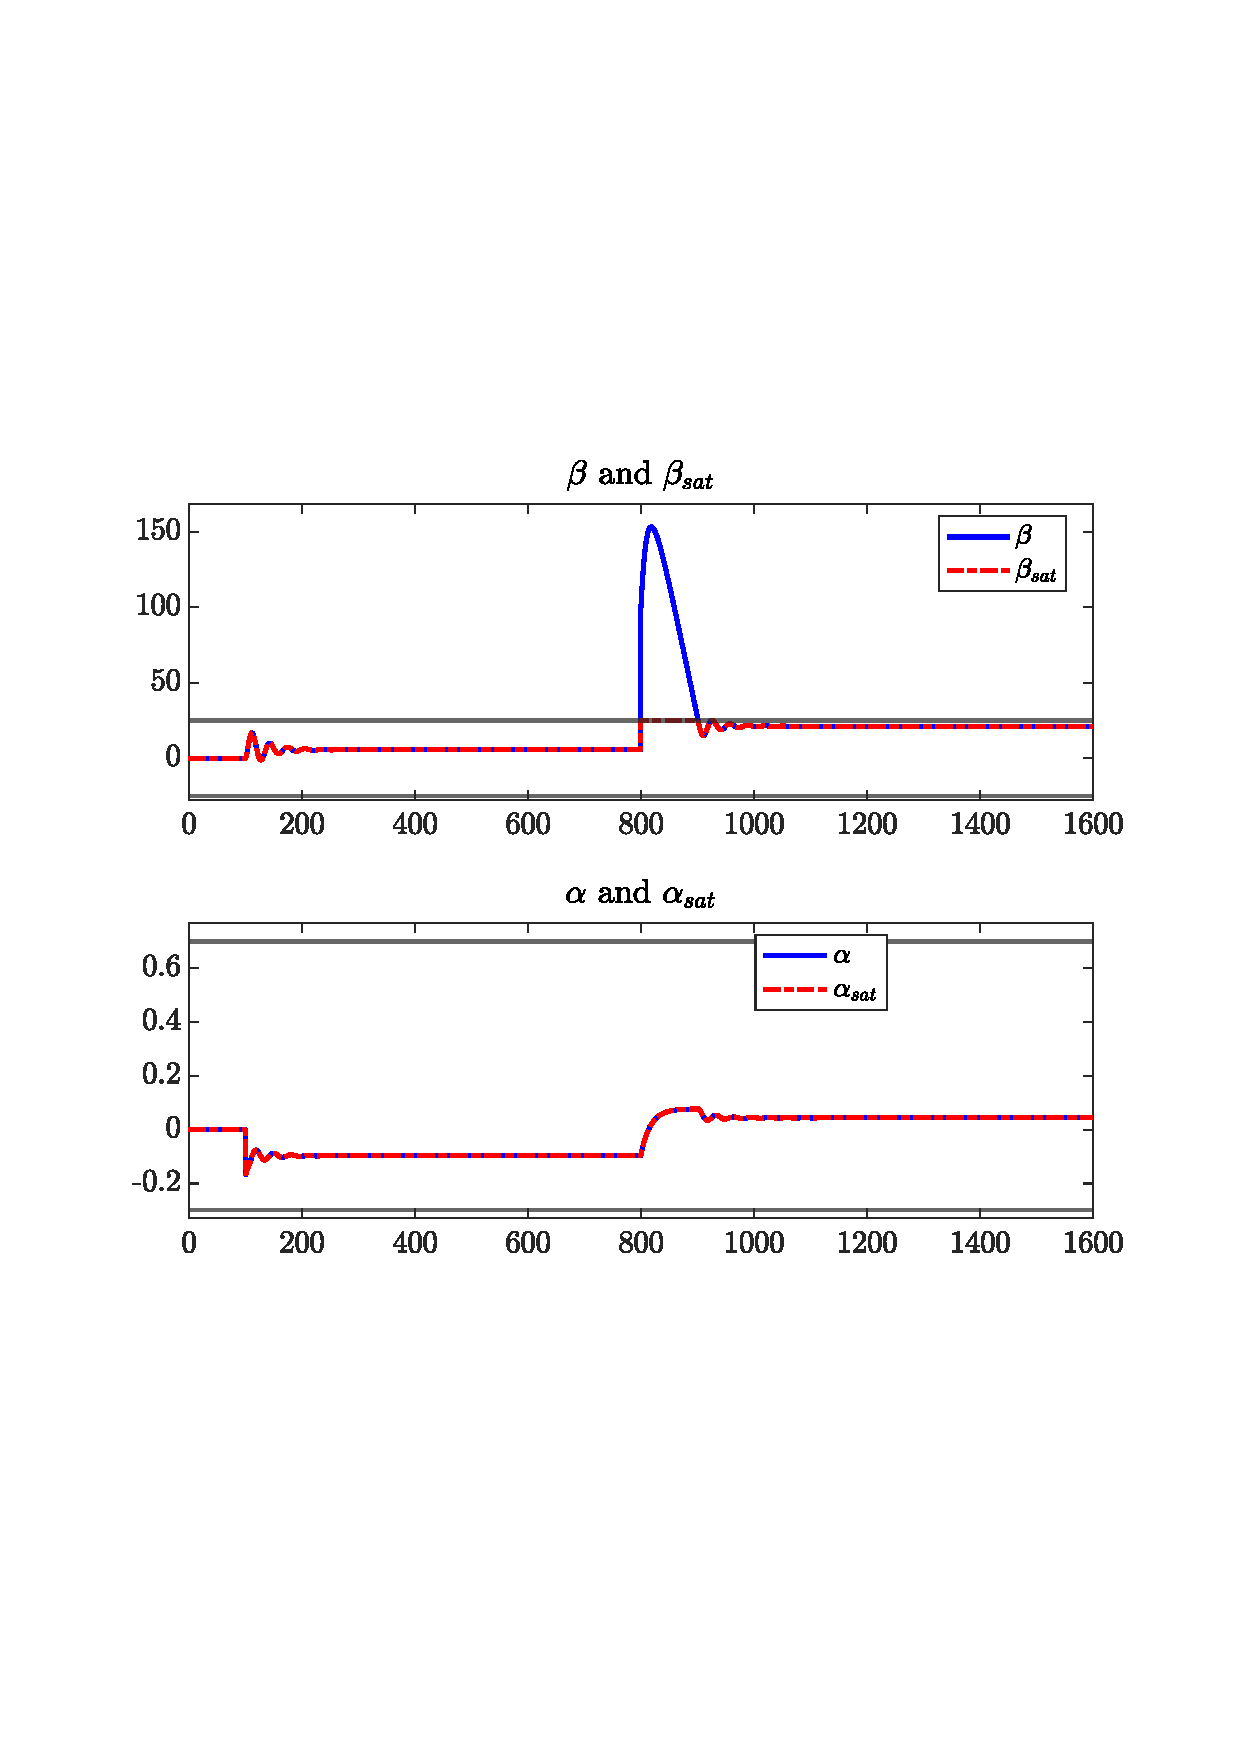
\includegraphics[width=1\linewidth, scale=1, trim=60 230 55 150,clip]{fig/Open_loop/exp_2_in.pdf}}

    \caption{Visualization of reference signal and the controller output for experiment 1 and experiment 2.}
    \label{fig:condes:results:benchmark_compare}
\end{figure}


We now compare the behaviour seen in \cite{Fragoso_et_al_2017} and in the presented results (\autoref{tab:condes:results:benchmark_changes}).
For the pitch angle the results can be duplicated.
When the set-point change is applied to $\omega_r$ the duty cycle $\alpha$ shows a different behaviour in terms of magnitude, but has the same sign.
Thus, global behaviour is also confirmed.
One reason for the deviation may also lie in the RGA.
Despite the different magnitude, the system can reach the same set-point with a small error.
It must be emphasised that all values are read from figures and deviations can occur in this process.


\begin{table}[H]
    \caption{Comparing behaviour from \cite{Fragoso_et_al_2017} and experiments 1 and 2.}
    \centering
    \begin{tabular}{ccccc} \toprule
        & \multicolumn{4}{c}{Results in } \\
        Set-point change & \multicolumn{2}{c}{Fragoso et~al.} & \multicolumn{2}{c}{This work} \\
        & $\beta$ & $\alpha$& $\beta$ & $\alpha$ \\ \midrule
        $P_g$ & \SI[retain-explicit-plus]{+10}{\degree} & $-10$ & \SI[retain-explicit-plus]{+10}{\degree} & $-10$ \\
        $\omega_r$ & \SI[retain-explicit-plus]{+20}{\degree} & $+15$ & \SI[retain-explicit-plus]{+20}{\degree}& $+5$\\ \bottomrule
    \end{tabular}
    \label{tab:condes:results:benchmark_changes}
\end{table}


\subsection{PID wind-up}

\autoref{sec:condes:implementation_simulink:closed_loop} already mentioned the \texttt{saturation}-block in the closed loop.
We know focus on the PID wind-up.
When wind-up occurs the controller is outputs a manipulated variable in an \textit{unrealistic} or physically impossible order of magnitude.
This signal is saturated.
Therefore the systems input signal is smaller than the controller output.
If the reference error is nonetheless not vanishing \textit{fast} enough the controller output is winding up.
Which can not be put through to the system because of the saturation.

We look at experiment 7.
In experiment 7 at $t=\SI{1200}{\second}$ the wind speed increases instantly from \SI{0}{\metre\per\second} to \SI{0.5}{\metre\per\second}.
The controller tries to concur this disturbance by increasing the pitch angle $\beta$.
Due to the saturation the controller can not \textit{act hard enough}.
The error increases and the controller increases the output (higher pitch angle).
The pitch angle exceed \SI{360}{\degree} multiple times, which is a physical not plausible behaviour.
There are several anti-wind-up strategies to prevent an increasing error.

\begin{figure}[H]
    \center
    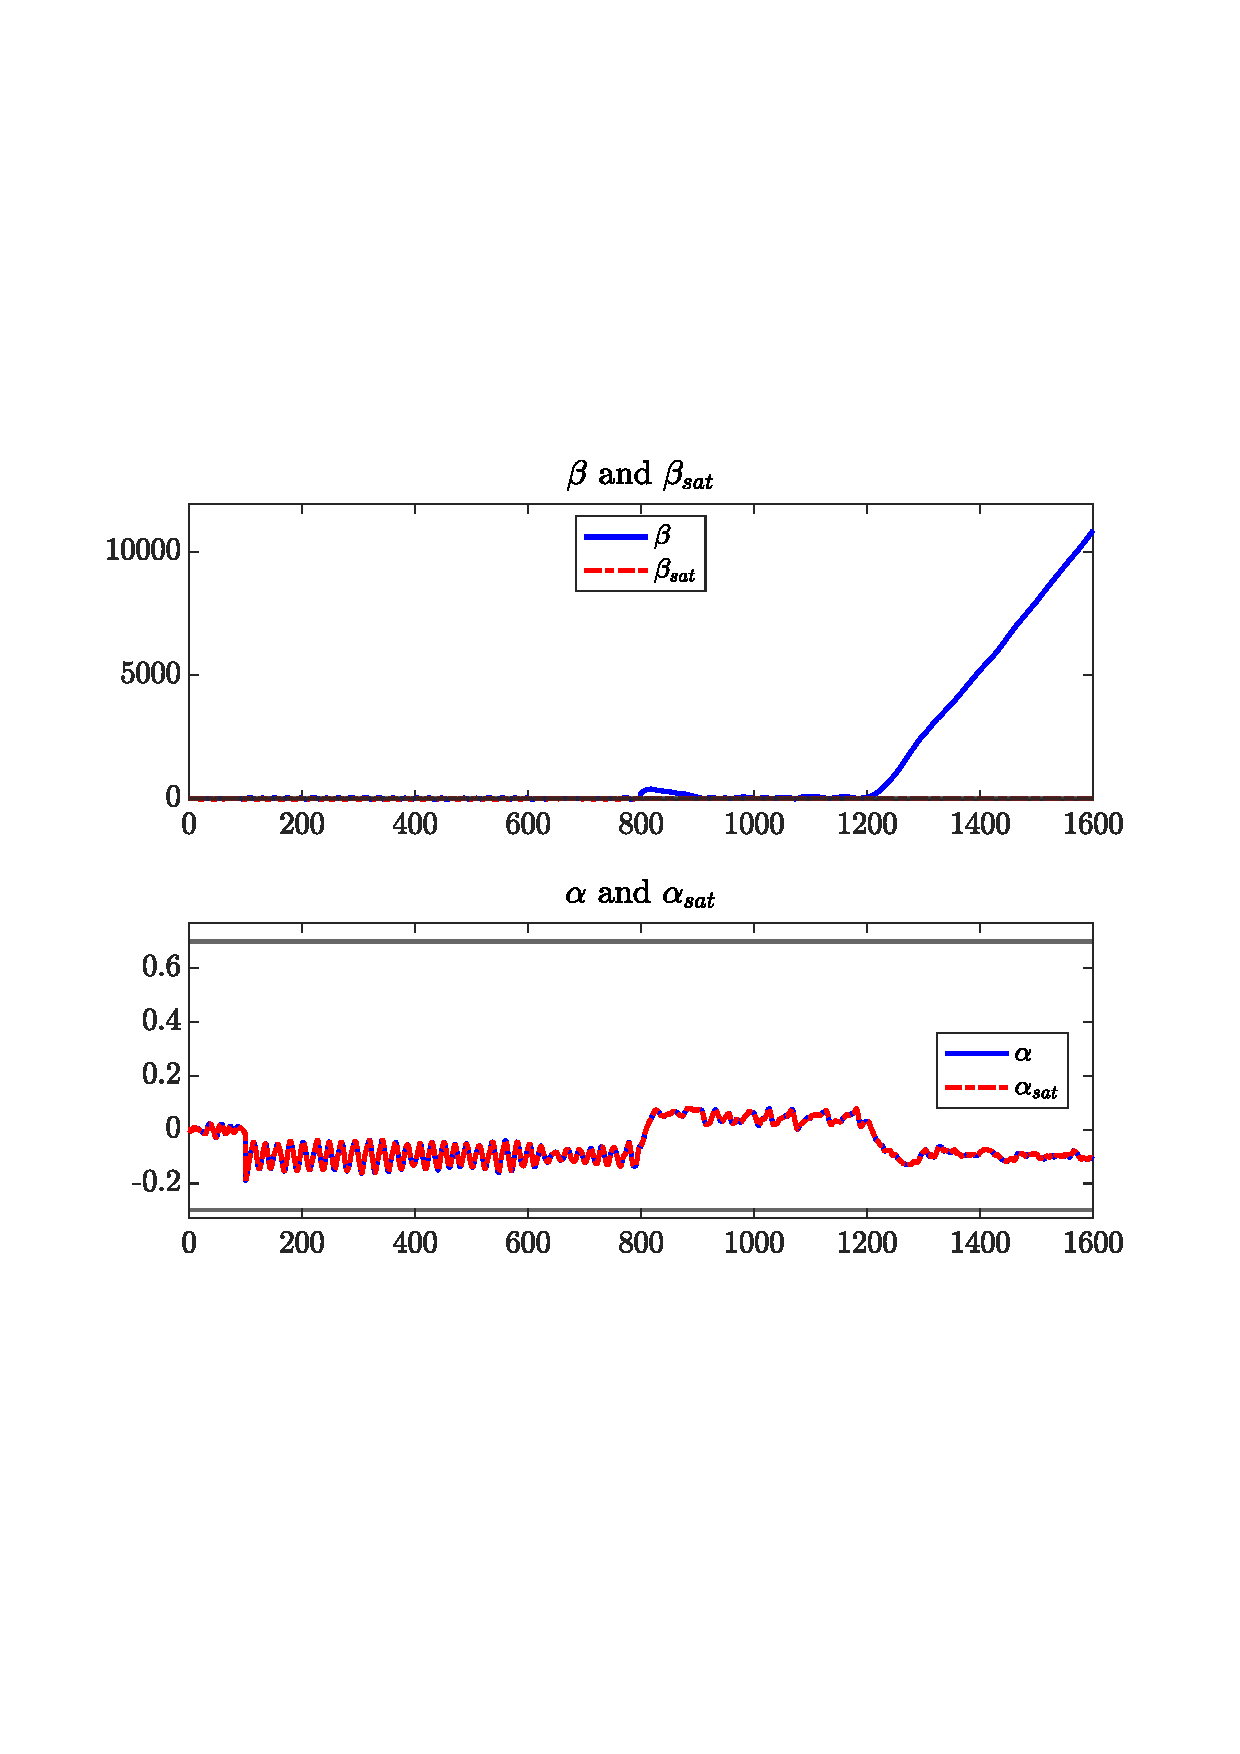
\includegraphics[width=0.7\linewidth, trim=50 230 55 180,clip]{fig/Open_loop/exp_7_in.pdf}
    \caption{Wind-up of a PID controller seen in experiment 7.}
    \label{fig:condes:results:wind_up}
\end{figure}


\subsection{Using controller outside of identified transfer function}

This subsections answers the question if a controller designed for a specific wind speed can be used in other \textit{wind speed domains}.
To answer the question a controller designed using transfer function at a wind speed of \SI{8}{\metre\per\second} is used with the identified system at a wind speed of \SI{7}{\meter\per\second}.
Looking at the results of experiments 3 and 4 and comparing it to the results of experiments 1 and 2, lead to the conclusion that a controller can be used \textit{outside} of its wind speed domain (\autoref{fig:condes:results:controller_outside_domain}).
Experiment 1 and experiment 3 use the same parameters, in experiment 3 only the controller is designed for a system with a wind speed of \SI{7}{\metre\per\second}, instead of \SI{8}{\metre\per\second}.
The same holds for the experiment pair 2 and 4.

In conclusion 

\begin{figure}[H]
    \centering

    \subcaptionbox{Exp. 1: Absolute error over time \label{fig:condes:results:exp1:error}}[.45\textwidth]{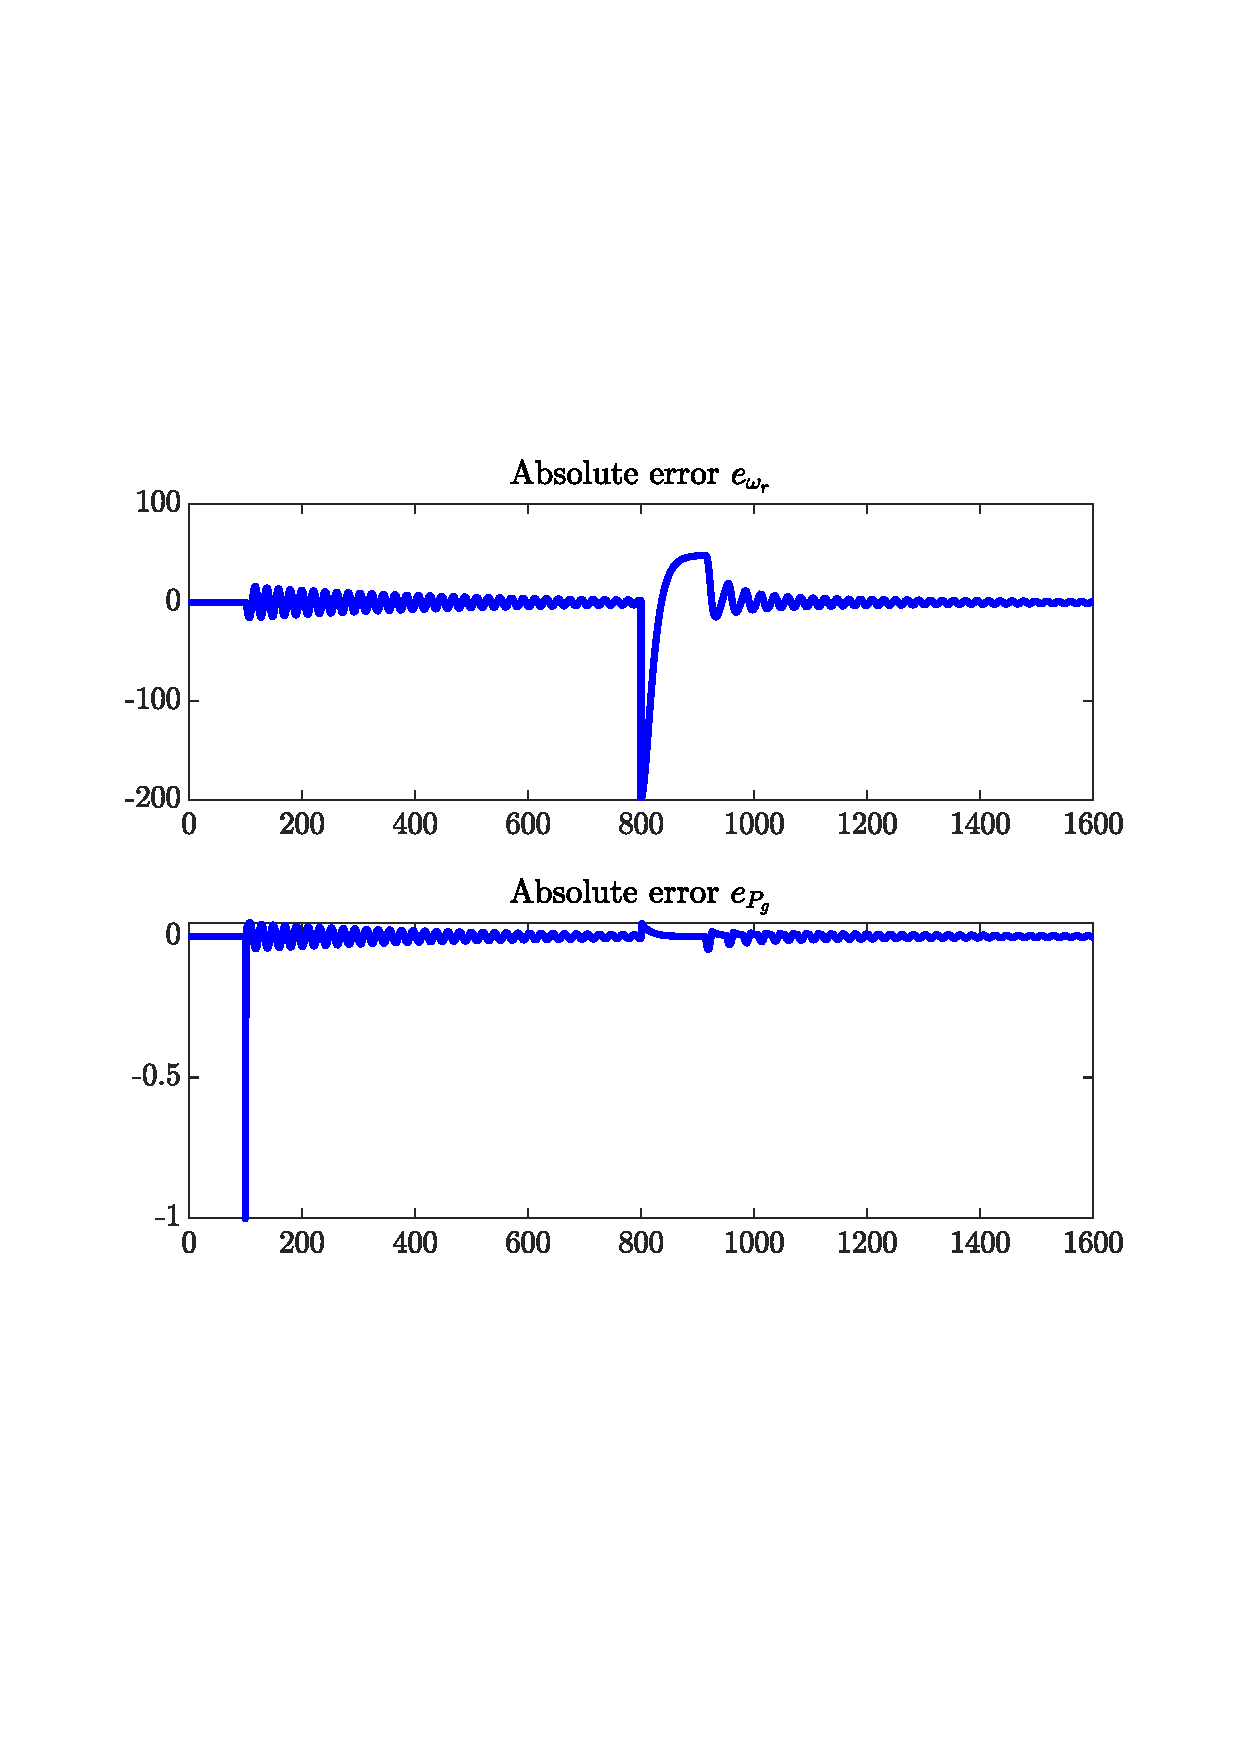
\includegraphics[width=1\linewidth, scale=1, trim=60 230 55 150,clip]{fig/Open_loop/exp_1_error.pdf}}
%
\subcaptionbox{Exp. 3: Absolute error over time \label{fig:condes:results:exp3:error}}[.45\textwidth]{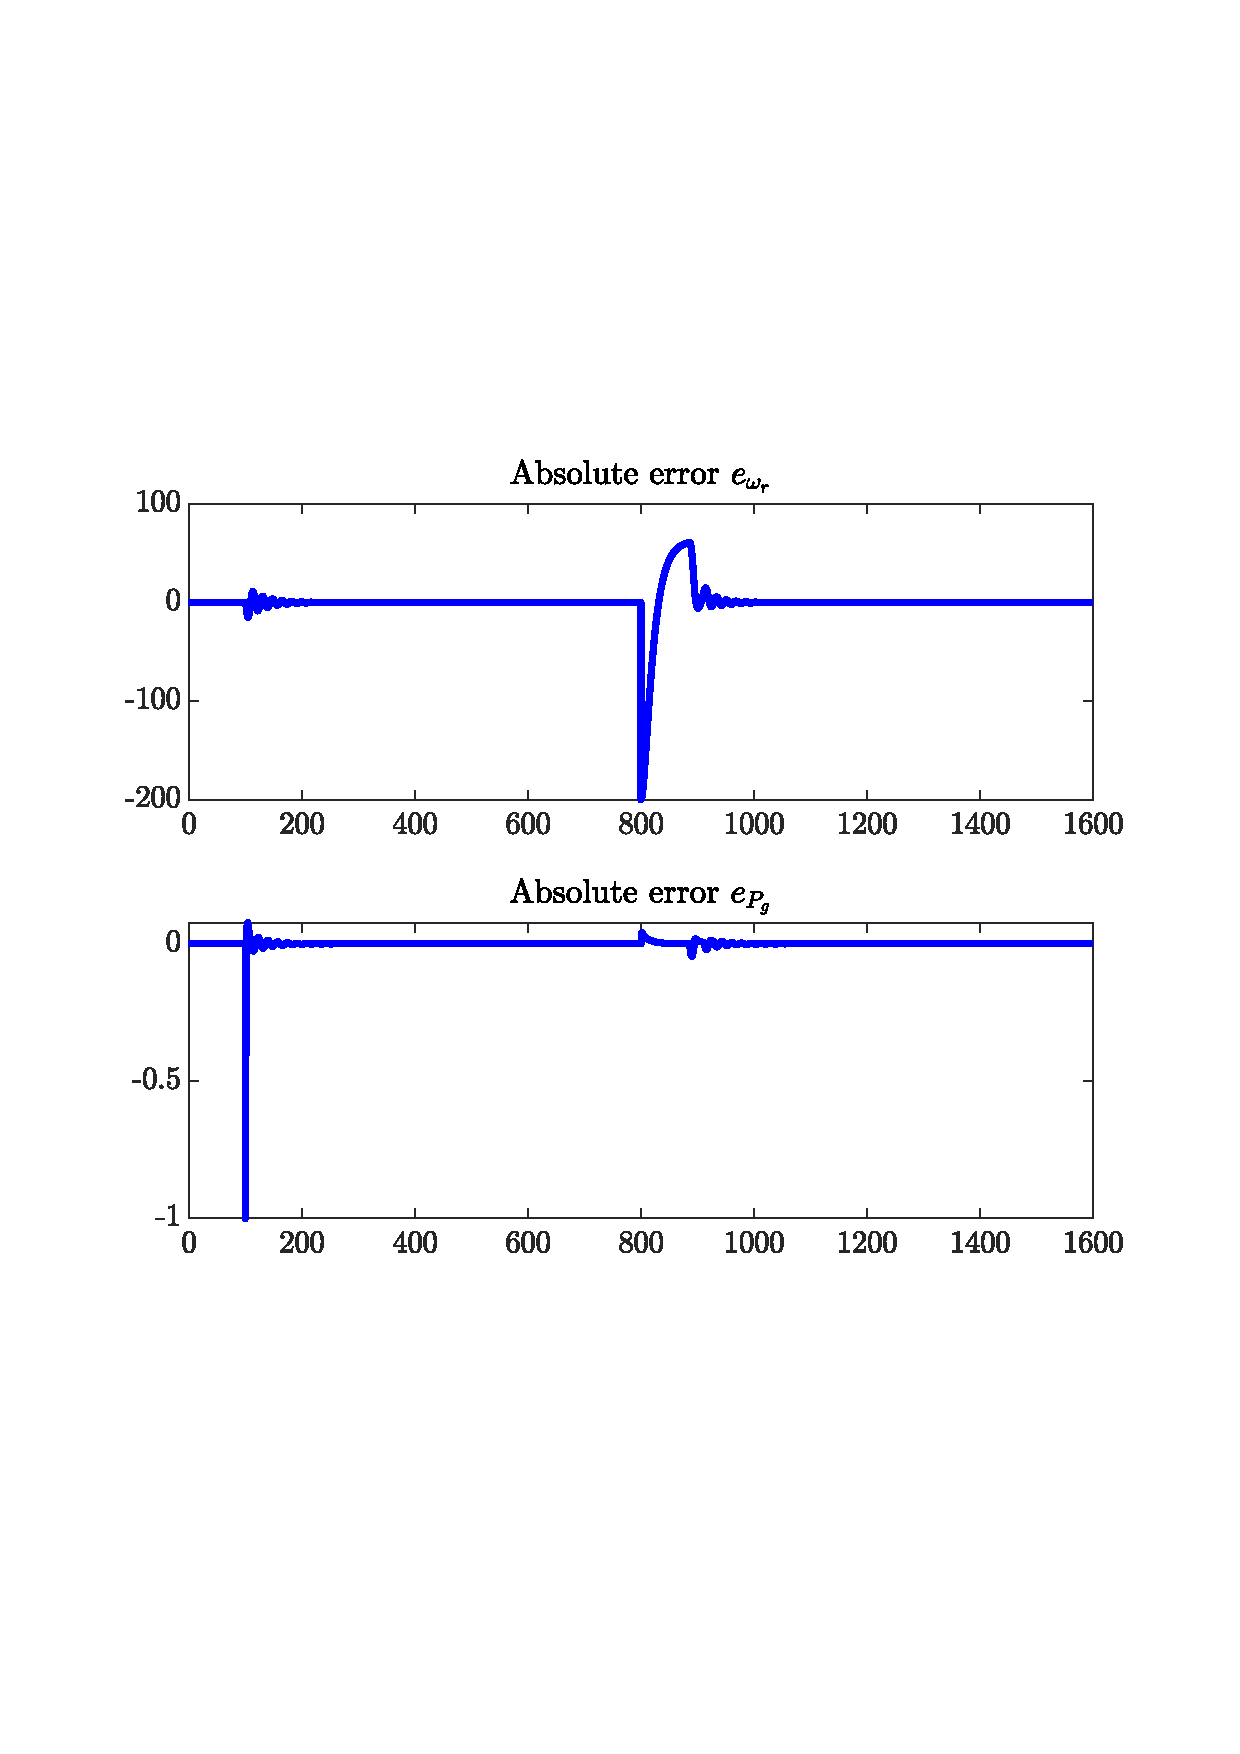
\includegraphics[width=1\linewidth, scale=1, trim=60 230 55 150,clip]{fig/Open_loop/exp_3_error.pdf}}
\\
    \subcaptionbox{Exp. 2: Absolute error over time \label{fig:condes:results:exp2:error}}[.45\textwidth]{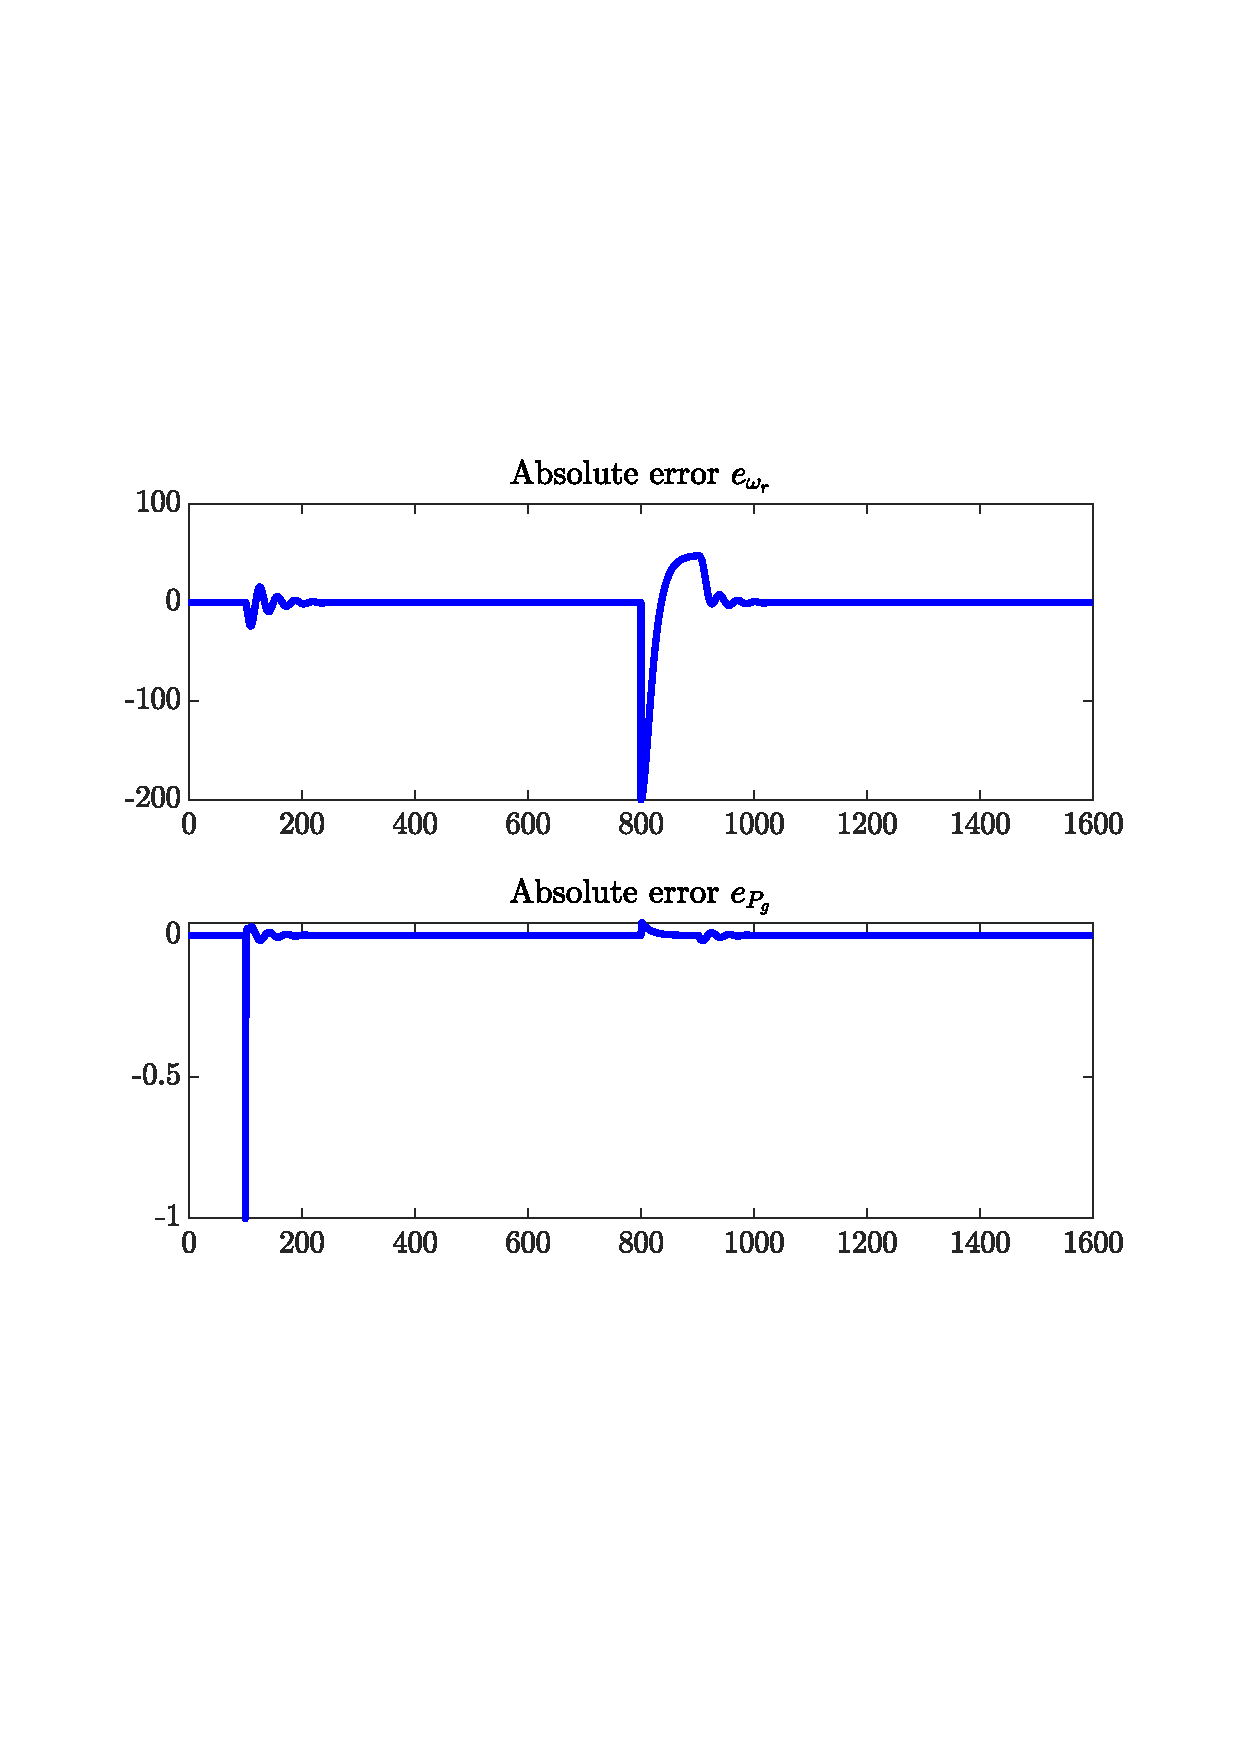
\includegraphics[width=1\linewidth, scale=1, trim=60 230 55 150,clip]{fig/Open_loop/exp_2_error.pdf}}
%
\subcaptionbox{Exp. 4:  Absolute error over time \label{fig:condes:results:exp4:error}}[.45\textwidth]{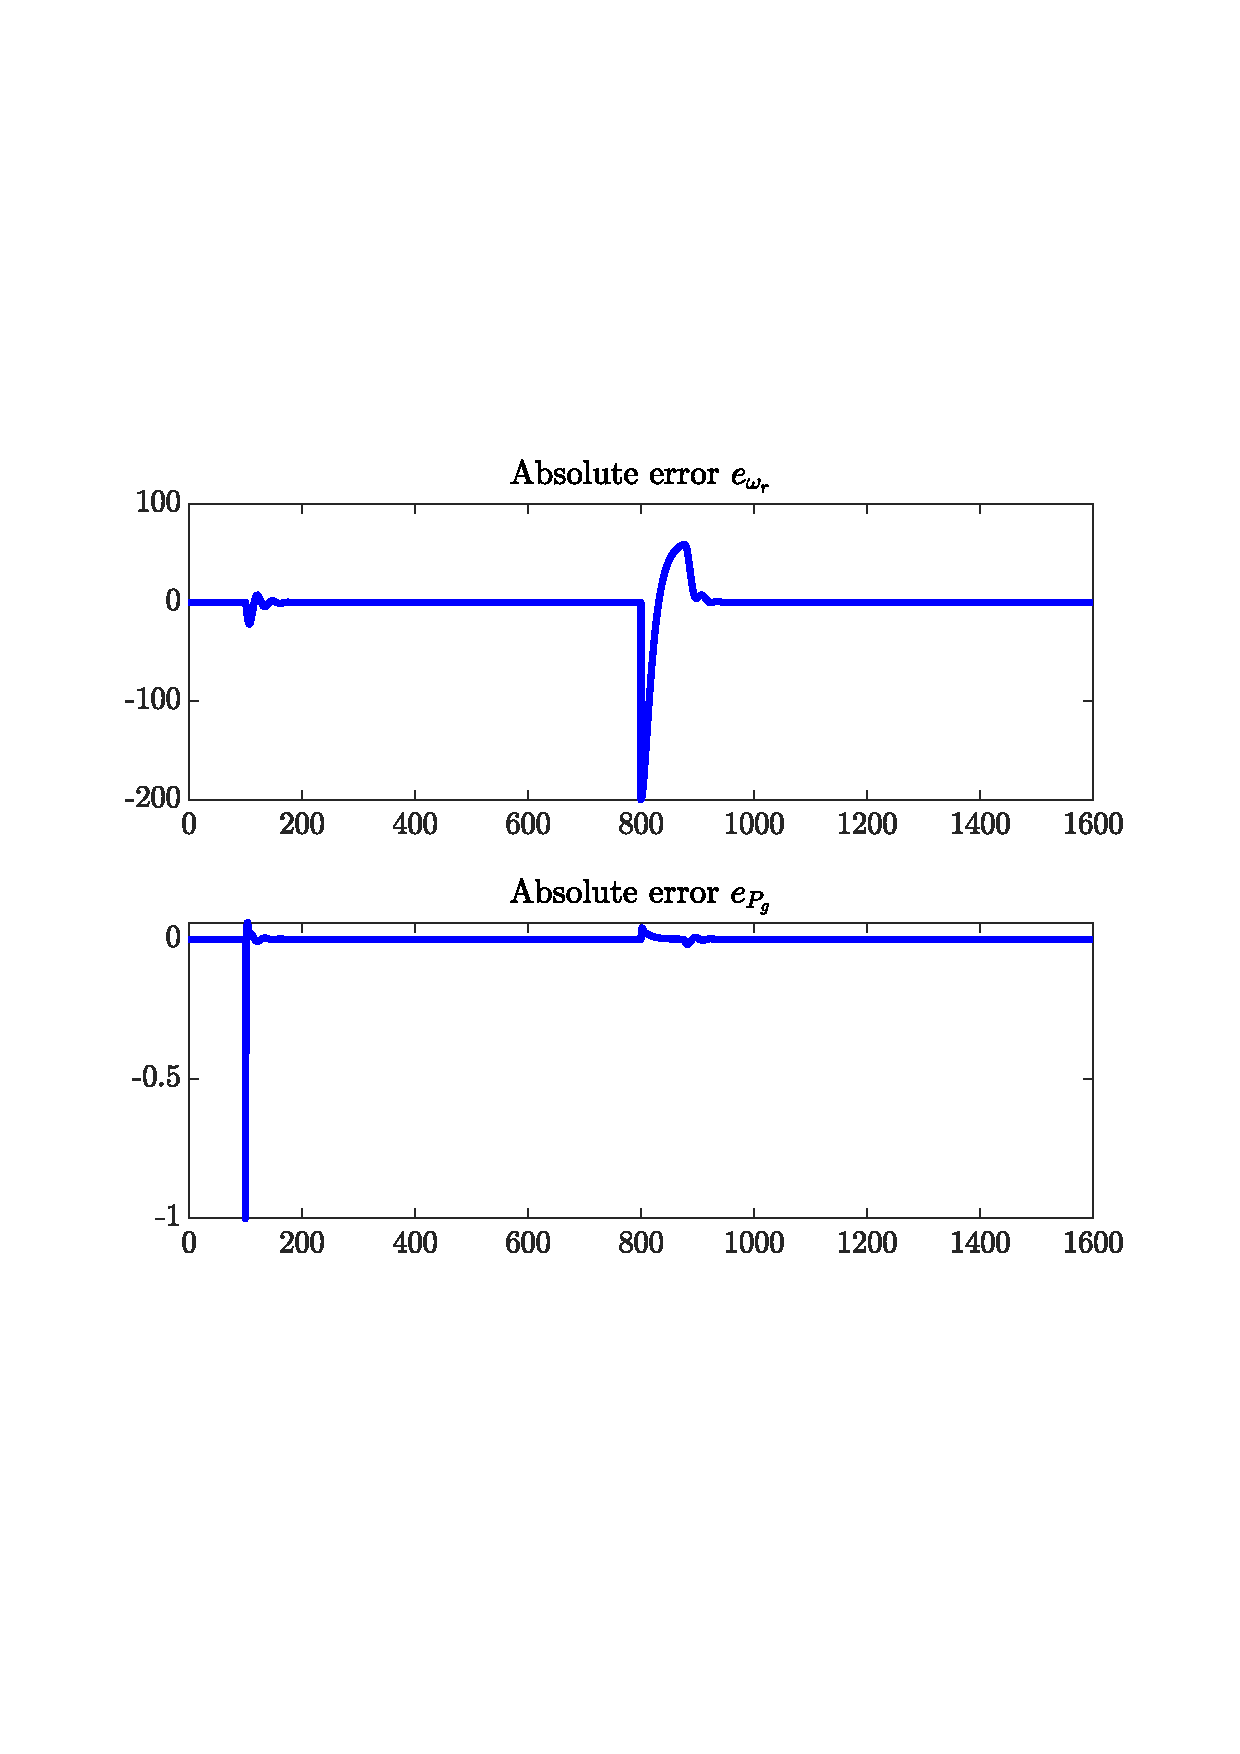
\includegraphics[width=1\linewidth, scale=1, trim=60 230 55 150,clip]{fig/Open_loop/exp_4_error.pdf}}

    \caption{Comparison of the time course of the absolute error for experiments 1 to 4.}
    \label{fig:condes:results:controller_outside_domain}
\end{figure}


\subsection{Introduction of noise}

For the first four experiments no noise was introduced.
For a real life application this a unrealistic scenario especially for a naturally occurring phenomena like wind.
To address this a white noise and lastly a step change (boe) is introduced.
This section focuses on the controllers capability to deal with noise.

We will look at the introduction of a white noise with a \textit{noise power} of $\xi= \SI{0.05}{\metre\per\second}$ (experiments 5 and 6) and analyze the controller output and the set-point derivation.

\begin{figure}[H]
    \centering

    \subcaptionbox{Exp. 5:  Disturbance and control variable\label{fig:condes:results:exp5:ref}}[.45\textwidth]{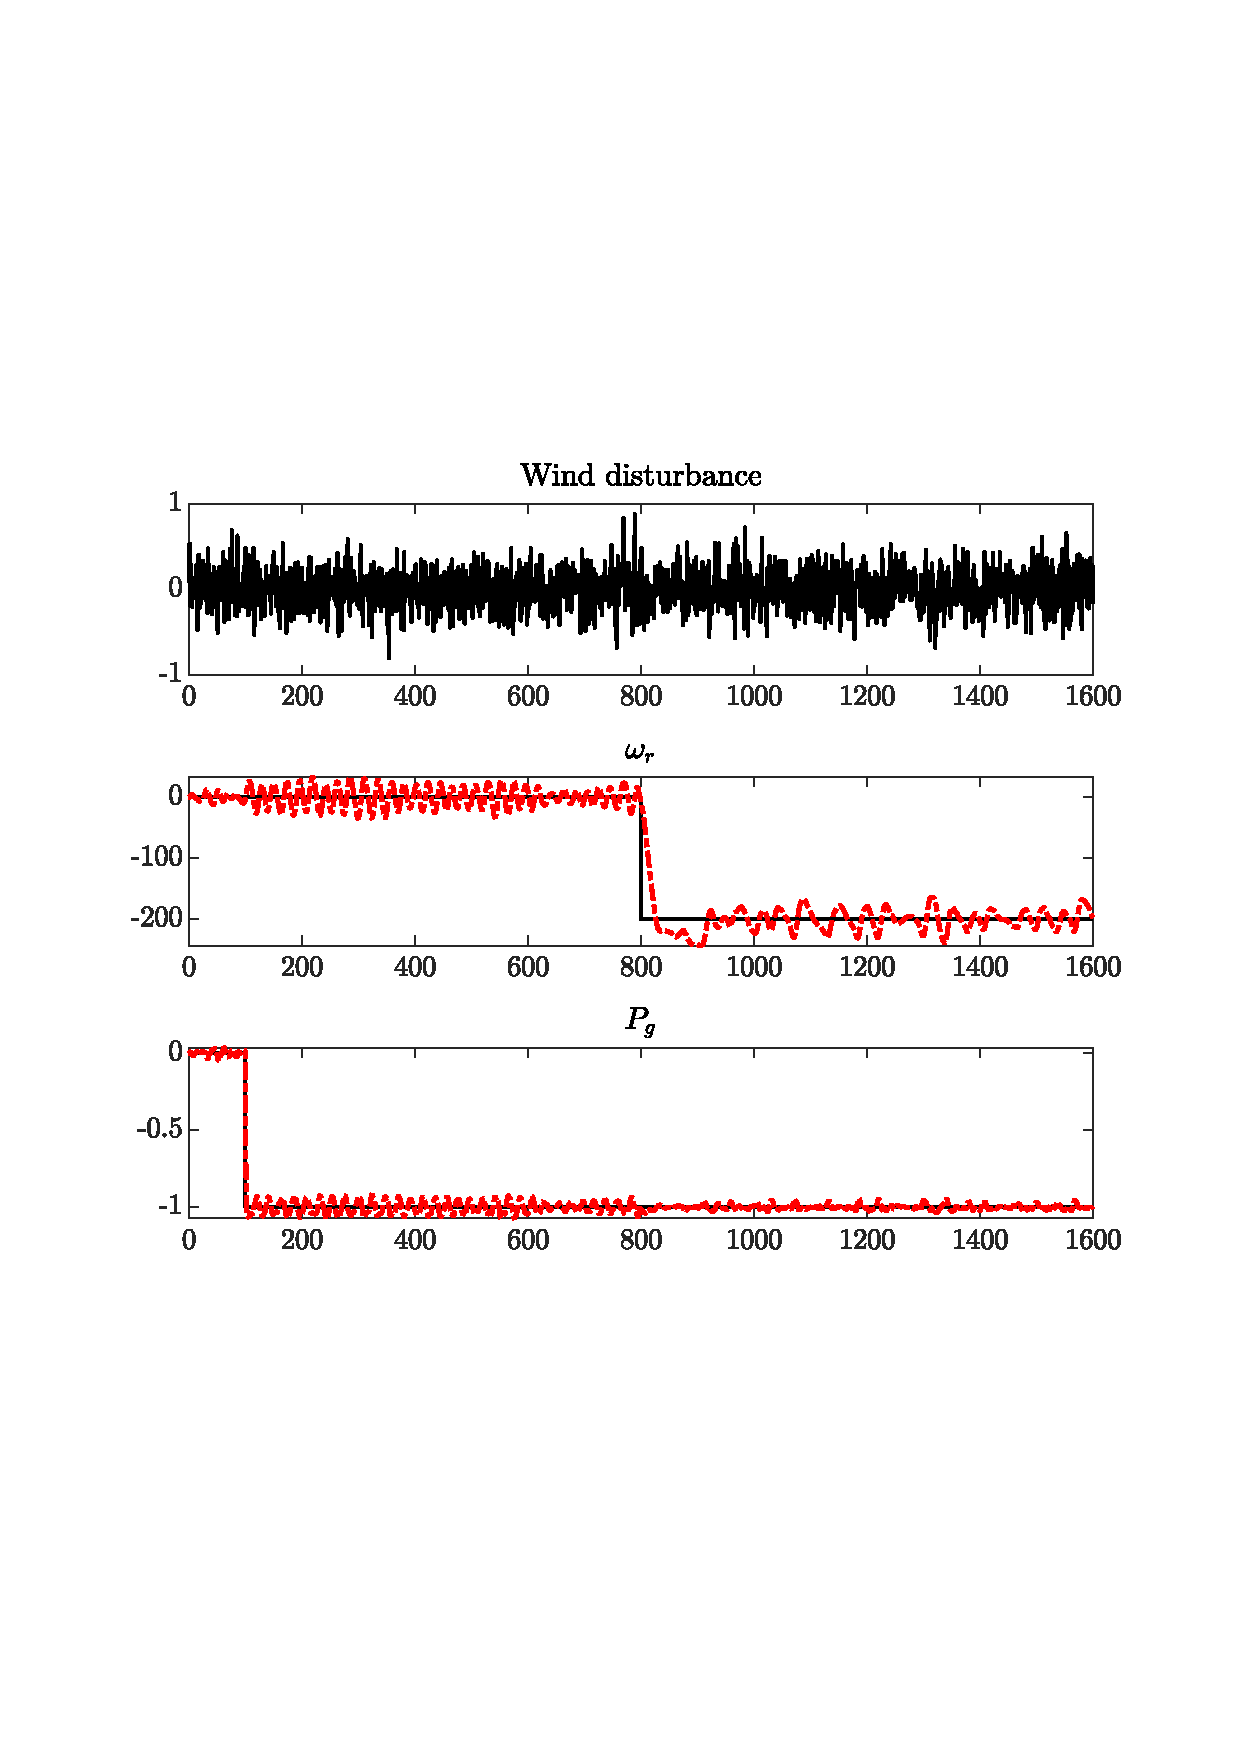
\includegraphics[width=1\linewidth, scale=1, trim=60 230 55 150,clip]{fig/Open_loop/exp_5_ref.pdf}}
%
\subcaptionbox{Exp. 6:  Disturbance and control variable \label{fig:condes:results:exp6:ref}}[.45\textwidth]{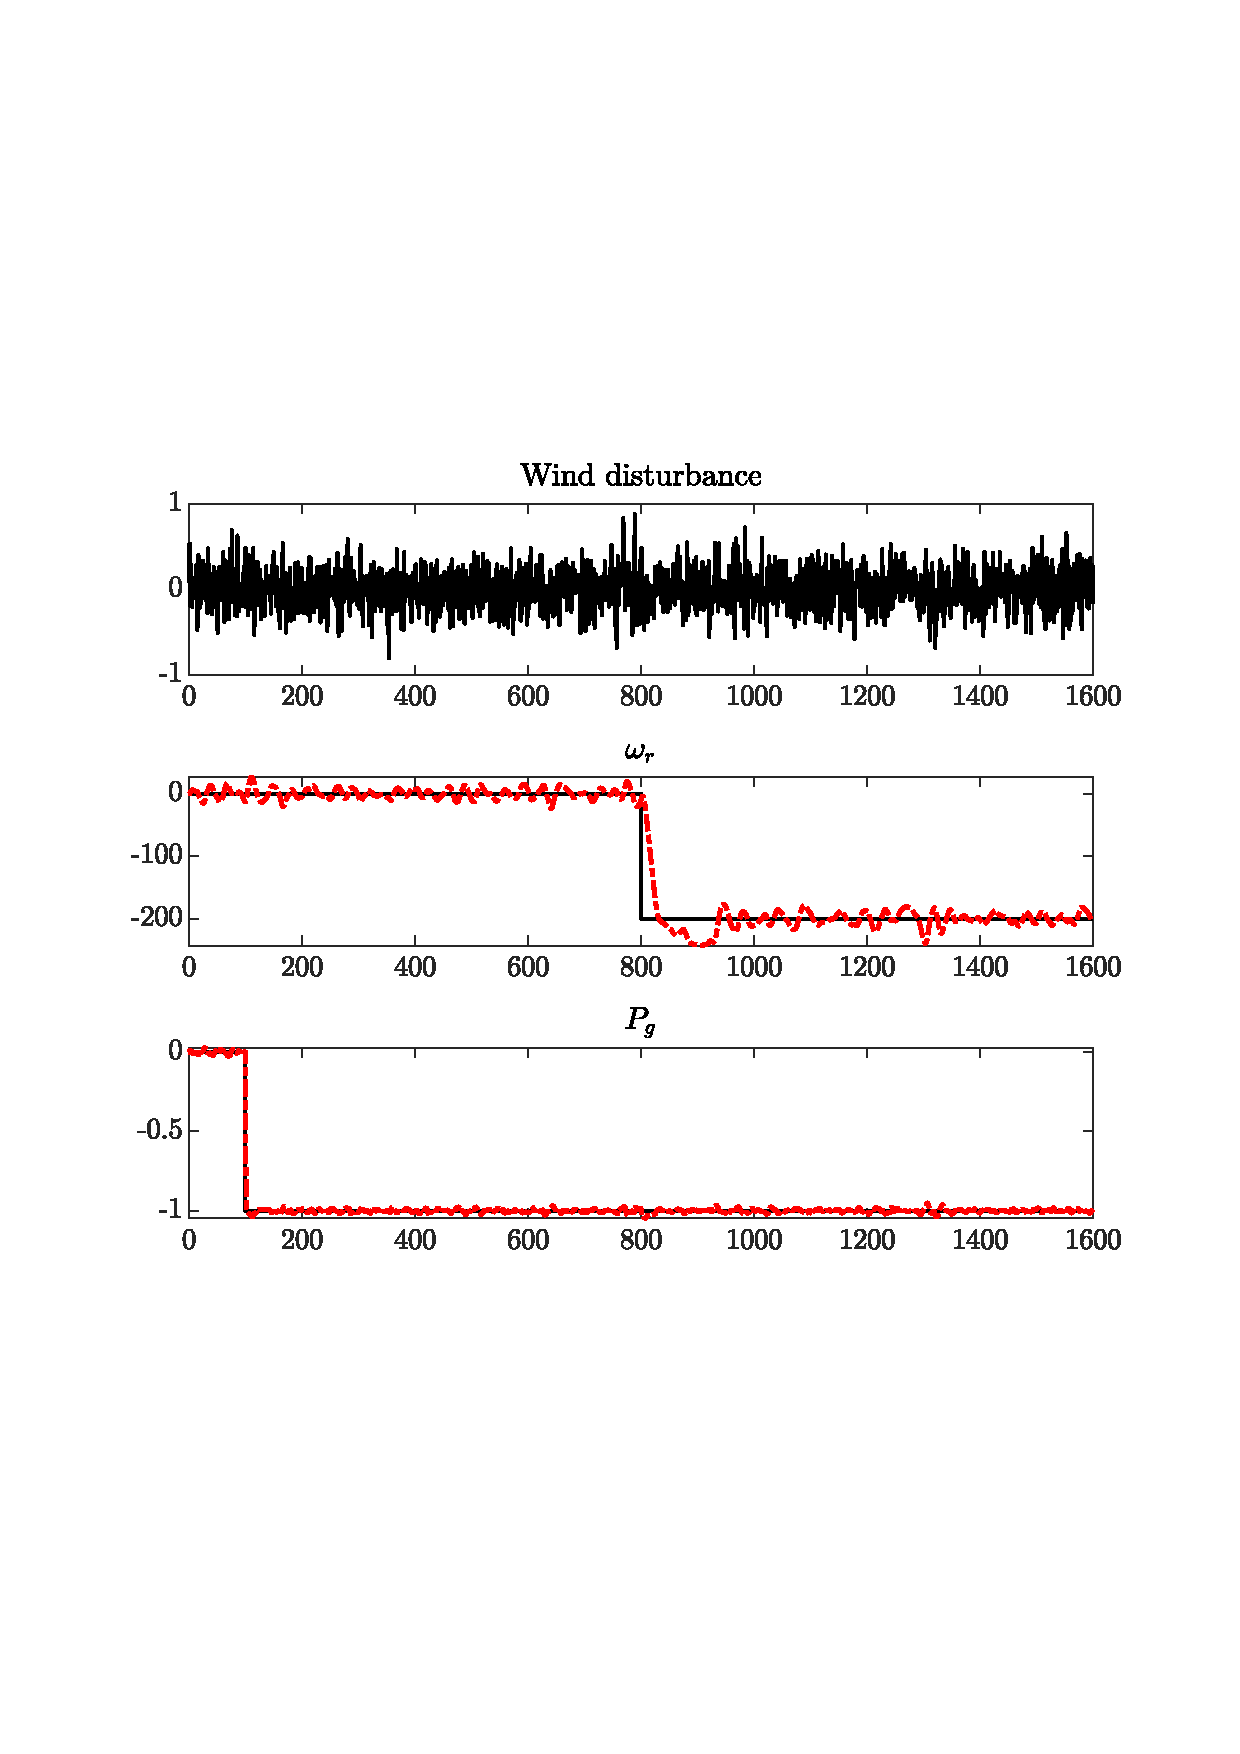
\includegraphics[width=1\linewidth, scale=1, trim=60 230 55 150,clip]{fig/Open_loop/exp_6_ref.pdf}}
\\
    \subcaptionbox{Exp. 5: Controlled variable \label{fig:condes:results:exp5:in}}[.45\textwidth]{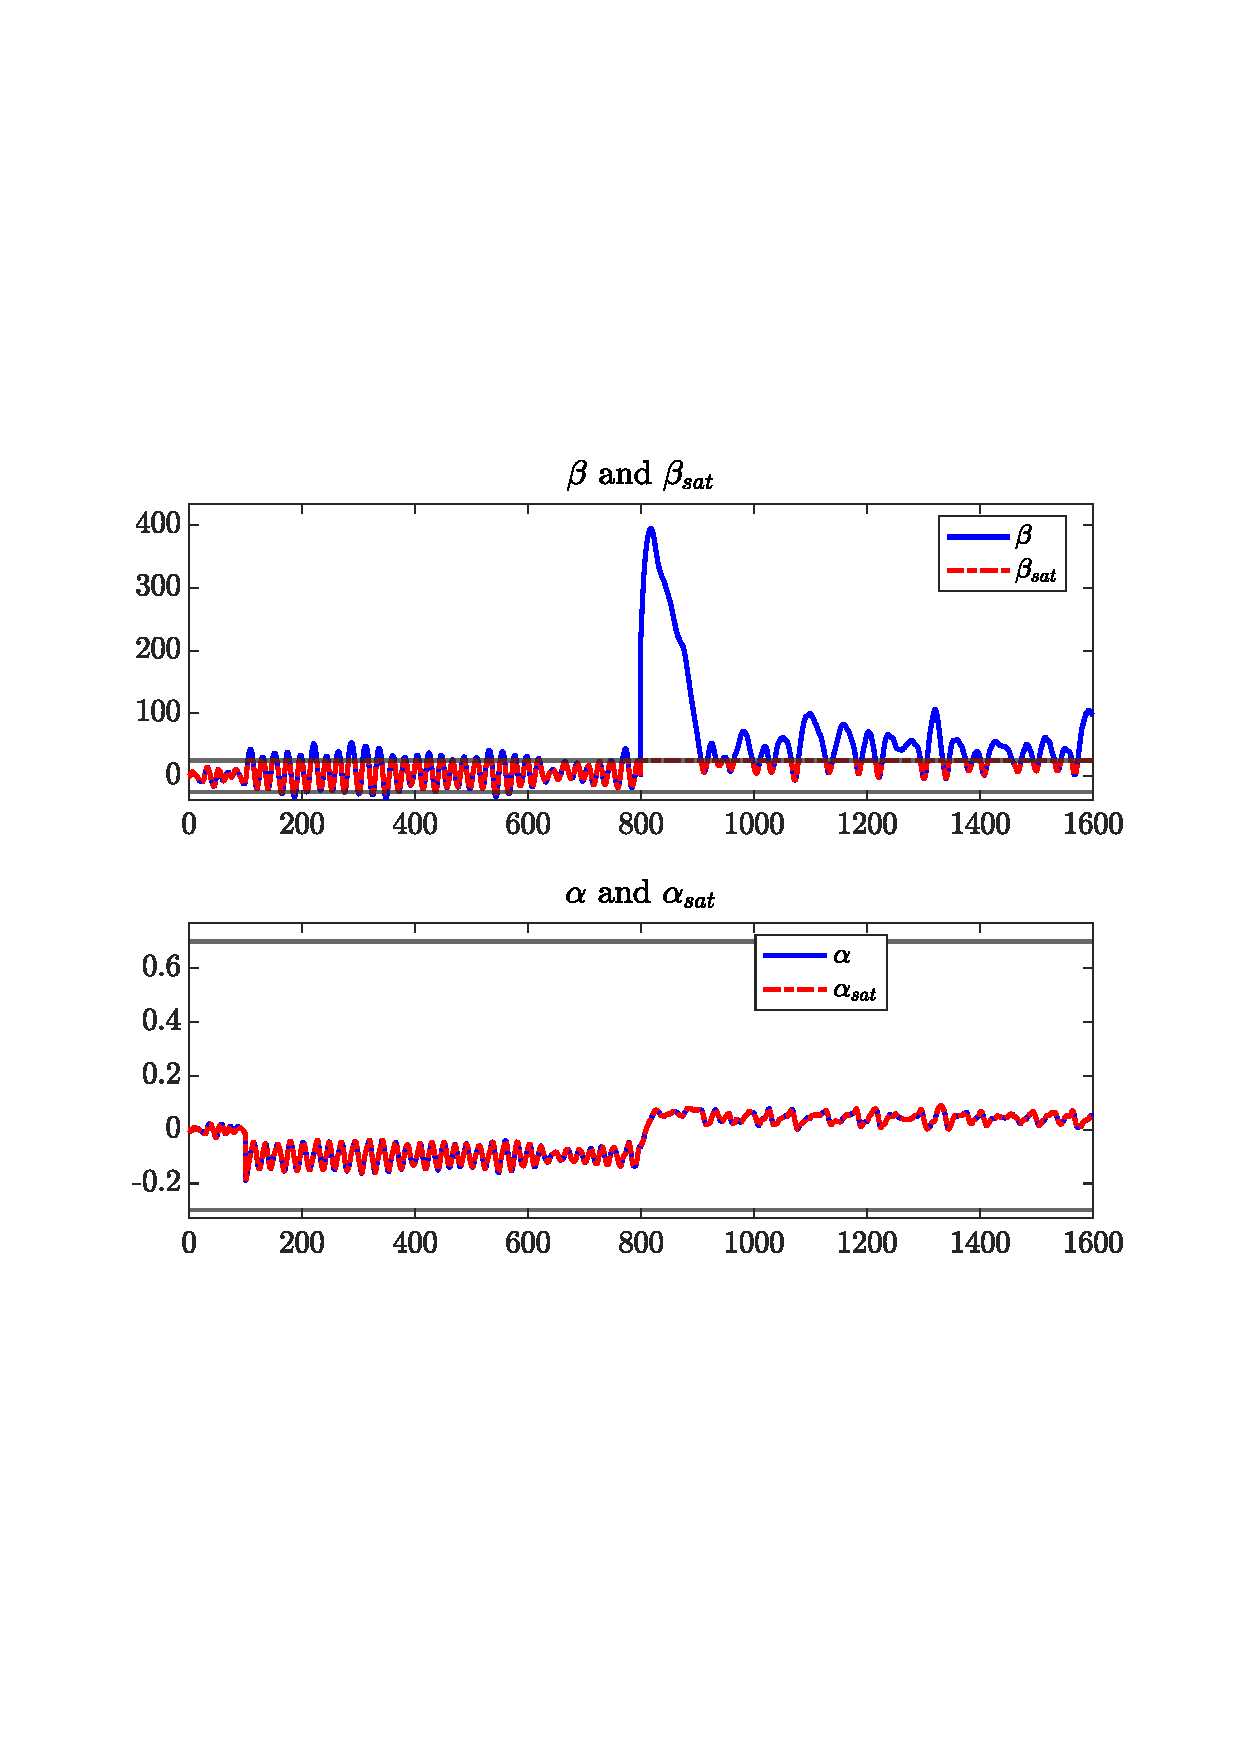
\includegraphics[width=1\linewidth, scale=1, trim=60 230 55 150,clip]{fig/Open_loop/exp_5_in.pdf}}
%
\subcaptionbox{Exp. 6:  Controlled variable \label{fig:condes:results:exp6:in}}[.45\textwidth]{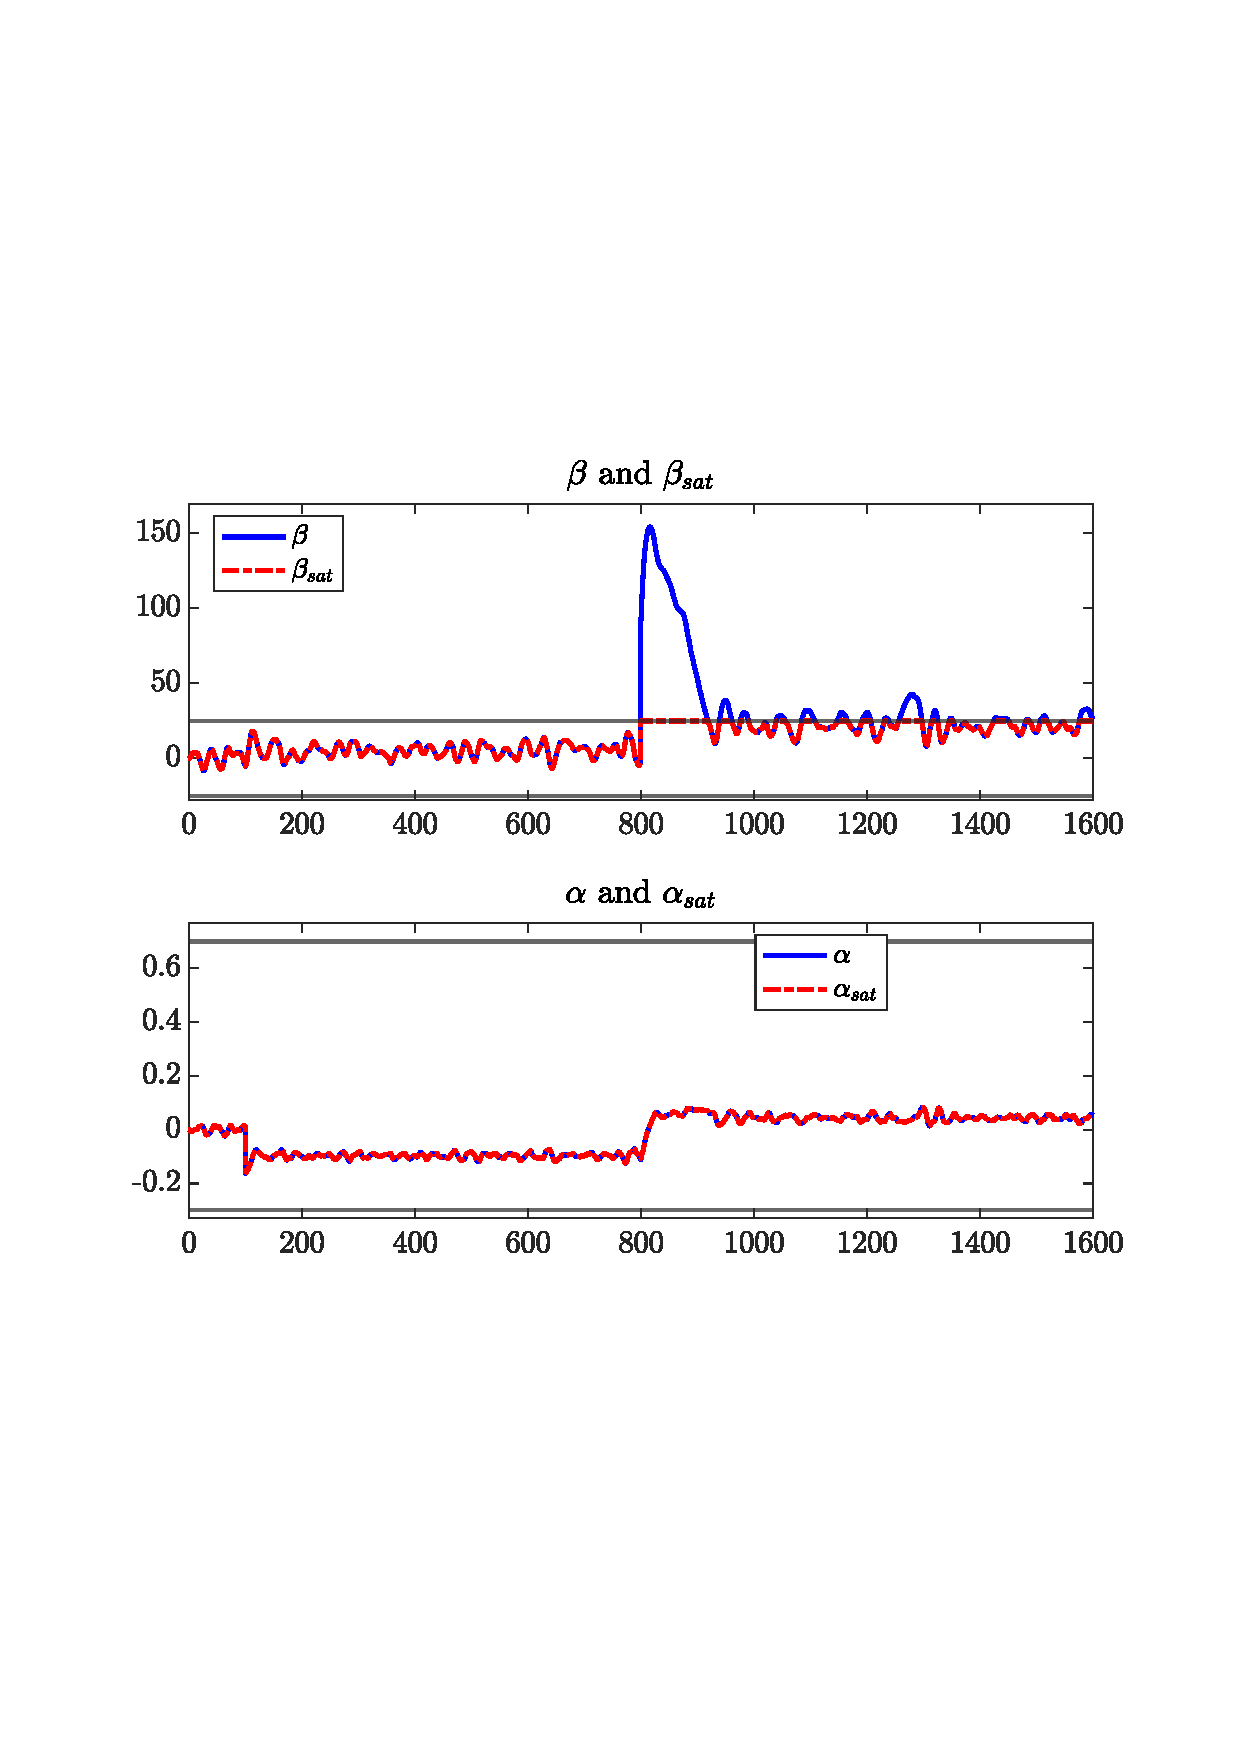
\includegraphics[width=1\linewidth, scale=1, trim=60 230 55 150,clip]{fig/Open_loop/exp_6_in.pdf}}

    \caption{Influence of white noise to controller performance}
    \label{fig:condes:results:intro_noise}
\end{figure}

Both controllers are showing good results.
Due to the high frequency of the white noise the controller reacts with many and also high frequent control inputs.
In a real life application this could cause problems.
A controller can not be arbitrarily fast with its outputs due to limitation in computation and especially of the actuators.
A blade can not change its pitch angle in \si{milli\second}, in particular for real blades, this would cause a great strain.
A filter could be used to filter the high frequent wind changes.


\subsection{Further steps}

Three main interests of further research can be identified.
The use of relay-feedback controller design could be investigated and compared to the published results.
Second, the implementation of noise could be made more realistic.
Realistic noise would model real-world wind behaviour better.
And third, the implementation of anti-wind-up strategies could increase the controller performance.
